% Copyright 2018-2019 Melvin Eloy Irizarry-Gelpí
\setcounter{chapter}{4}
\chapter{Capacitors and Inductors}
%%%%%%%%%%%%%%%%%%%%%%%%%%%%%%%%%%%%%%%%%%%%%%%%%%%%%%%%%%%%%%%%%%%%%%%%%%%%%%%%
In this experiment you will learn about circuits with capacitors and inductors.
%%%%%%%%%%%%%%%%%%%%%%%%%%%%%%%%%%%%%%%%%%%%%%%%%%%%%%%%%%%%%%%%%%%%%%%%%%%%%%%%
\section{Preliminary}
%%%%%%%%%%%%%%%%%%%%%%%%%%%%%%%%%%%%%%%%%%%%%%%%%%%%%%%%%%%%%%%%%%%%%%%%%%%%%%%%
A given component in an electric circuit can have many physical properties. Among them are resistance, capacitance, and inductance.
%%%%%%%%%%%%%%%%%%%%%%%%%%%%%%%%%%%%%%%%%%%%%%%%%%%%%%%%%%%%%%%%%%%%%%%%%%%%%%%%
\subsection{Resistance and Resistors}
%%%%%%%%%%%%%%%%%%%%%%%%%%%%%%%%%%%%%%%%%%%%%%%%%%%%%%%%%%%%%%%%%%%%%%%%%%%%%%%%
By now, electrical \textbf{resistance} should be familiar. The \textbf{SI unit} for electrical resistance is the \textbf{ohm}:
\begin{equation}
	1 \text{ ohm} = 1\;\Omega = 1 \text{ V/A}
\end{equation}
Here, V is volt (voltage) and A is ampere (current). A component in a circuit with a fixed amount of resistance is called a \textbf{resistor}. The mathematical symbol for resistance is $R$.
%%%%%%%%%%%%%%%%%%%%%%%%%%%%%%%%%%%%%%%%%%%%%%%%%%%%%%%%%%%%%%%%%%%%%%%%%%%%%%%%
\subsection{Capacitance and Capacitors}
%%%%%%%%%%%%%%%%%%%%%%%%%%%%%%%%%%%%%%%%%%%%%%%%%%%%%%%%%%%%%%%%%%%%%%%%%%%%%%%%
Another important property is \textbf{capacitance}. The \textbf{SI unit} for capacitance is the \textbf{farad}:
\begin{equation}
	1 \text{ farad} = 1 \text{ F} = 1 \text{ C/V}
\end{equation}
Here, C is coulomb (electric charge) and V is volt (voltage). In some ways, capacitance measures the amount of electric charge needed to sustain an electric potential difference (i.e. a voltage). The mathematical symbol for capacitance is $C$.

A component in a circuit with a fixed amount of capacitance is called a \textbf{capacitor}. You can think of a capacitor as two parallel plates of conducting material where equal but opposite amounts of electric charge can accumulate.
%%%%%%%%%%%%%%%%%%%%%%%%%%%%%%%%%%%%%%%%%%%%%%%%%%%%%%%%%%%%%%%%%%%%%%%%%%%%%%%%
\subsection{Inductance and Inductors}
%%%%%%%%%%%%%%%%%%%%%%%%%%%%%%%%%%%%%%%%%%%%%%%%%%%%%%%%%%%%%%%%%%%%%%%%%%%%%%%%
The last property is \textbf{inductance}, which is like a magnetic cousin of capacitance. The \textbf{SI unit} for inductance is the \textbf{henry}:
\begin{equation}
	1 \text{ henry} = 1 \text{ H} = 1 \text{ T}\cdot\text{m}^{2}\text{/A}
\end{equation}
Here, T is tesla (magnetic field), m$^{2}$ is square meter (area), and A is ampere (current). Recall that the tesla unit is equivalent to
\begin{equation}
    1 \text{ T} = 1 \text{ V} \cdot \text{s/m}^{2}
\end{equation}
Thus, the henry unit is equivalent to:
\begin{equation}
    1 \text{ H} = 1 \text{ V}\cdot\text{s/A}
\end{equation}
In some ways, inductance measures the amount of voltage that arises per unit rate of change of electric current with time. The mathematical symbol for inductance is $L$.

A component in a circuit with a fixed amount of inductance is called an \textbf{inductor}. You can think of an inductor as a solenoid coil with a given amount of loops, with each loop enclosing some amount of area.
%%%%%%%%%%%%%%%%%%%%%%%%%%%%%%%%%%%%%%%%%%%%%%%%%%%%%%%%%%%%%%%%%%%%%%%%%%%%%%%%
\subsection{Exponential Decay Function}
%%%%%%%%%%%%%%%%%%%%%%%%%%%%%%%%%%%%%%%%%%%%%%%%%%%%%%%%%%%%%%%%%%%%%%%%%%%%%%%%
Before discussing the behavior of current and voltage in circuits with capacitors and inductors, it will be good to review the exponential decay function:
\begin{equation}
    \exp(-t) = e^{-t}
\end{equation}
Here, $e$ is the \textbf{natural base}:
\begin{equation}
    e = 2.71828...
\end{equation}
When $t = 0$, the exponential decay function gives
\begin{equation}
    \exp(0) = 1
\end{equation}
For large values of $t$, the exponential decay function approaches 0:
\begin{equation}
    \exp(-\infty) = 0
\end{equation}
In between $t = 0$ and $t \rightarrow \infty$ you have smaller and smaller values approaching zero.

The exponential decay function is an example of a function that is always positive, and always \textbf{decreasing} towards zero:
\begin{align}
    f(t) = \exp(-t) && 0 < f(t) \leq 1 && 0 \leq t < \infty
\end{align}
Multiplying the exponential decay function by a negative sign produces a function that is always negative, and always \textbf{increasing} towards zero:
\begin{align}
    g(t) = -\exp(-t) && -1 \leq g(t) < 0 && 0 \leq t < \infty
\end{align}
Another important combination is shifting vertically by 1, which gives a function that is always positive, and always \textbf{increasing} towards one:
\begin{align}
    h(t) = 1 - \exp(-t) && 0 \leq h(t) < 1 && 0 \leq t < \infty
\end{align}
Figures \ref{figure.05.f}, \ref{figure.05.g}, and \ref{figure.05.h} provide charts for these three functions.
%%%%%%%%%%%%%%%%%%%%%%%%%%%%%%%%%%%%%%%%%%%%%%%%%%%%%%%%%%%%%%%%%%%%%%%%%%%%%%%%
\subsection{Resistor and Capacitor in Series}
%%%%%%%%%%%%%%%%%%%%%%%%%%%%%%%%%%%%%%%%%%%%%%%%%%%%%%%%%%%%%%%%%%%%%%%%%%%%%%%%
A circuit with a resistor, a capacitor, and a direct-current (DC) source is called an \textbf{RC circuit}. In the simplest RC circuit, the resistor and capacitor are connected in series to the DC source via a particular switch.
%%%%%%%%%%%%%%%%%%%%%%%%%%%%%%%%%%%%%%%%%%%%%%%%%%%%%%%%%%%%%%%%%%%%%%%%%%%%%%%%
\subsubsection{Charging the Capacitor}
%%%%%%%%%%%%%%%%%%%%%%%%%%%%%%%%%%%%%%%%%%%%%%%%%%%%%%%%%%%%%%%%%%%%%%%%%%%%%%%%
When the switch is on, and the circuit is complete, the DC source pushes charges out into the circuit in the form of a current. This current causes positive electric charges to accumulate on one of the terminals of the capacitor, and negative electric charges on the other terminal of the capacitor. But the amount of electric charge $Q$ on the capacitor does not increase indefinitely: It settles on a maximum value $Q_{\infty}$. The particular manner in which the amount of \textbf{electric charge} on the capacitor increases with time is an example of an \textbf{exponential} increase:
\begin{equation}
    Q(t) = Q_{\infty} \left[ 1 - \exp\left(-\frac{t}{\tau_{C}}\right) \right]
    \label{eq.05.RC.q.charging}
\end{equation}
Here $Q_{\infty}$ is the amount of charge accumulated on the capacitor after an infinite amount of time, and $t$ correspond to the amount of time after the switch has been opened (the switch is opened at $t = 0$). The amount of \textbf{current} corresponds to the rate of change of the electric charge with time:
\begin{equation}
    I(t) = I_{0} \exp\left(-\frac{t}{\tau_{C}}\right)
    \label{eq.05.RC.i.charging}
\end{equation}
For a capacitor with capacitance $C$, the amount of \textbf{voltage} $V_{C}$ across the \textbf{capacitor} is directly proportional to the amount of electric charge accumulated on the capacitor:
\begin{equation}
    V_{C}(t) = \frac{Q(t)}{C} = V_{\infty} \left[ 1 - \exp\left(-\frac{t}{\tau_{C}}\right) \right]
    \label{eq.05.RC.vC.charging}
\end{equation}
The \textbf{voltage} $V_{R}$ across the \textbf{resistor} is directly proportional the the amount of current, via Ohm's law:
\begin{equation}
    V_{R}(t) = R I(t) = V_{\infty} \exp\left(-\frac{t}{\tau_{C}}\right)
    \label{eq.05.RC.vR.charging}
\end{equation}
Here, $V_{\infty}$ is related to $Q_{\infty}$ and/or $I_{0}$ via
\begin{eqnarray}
    V_{\infty} = \frac{Q_{\infty}}{C} = I_{0} R
\end{eqnarray}
The value of $V_{\infty}$ should correspond to the steady voltage across the DC source.

As you can see from (\ref{eq.05.RC.q.charging}), (\ref{eq.05.RC.i.charging}), and (\ref{eq.05.RC.vC.charging}), the amount of charge, current and voltage related to a capacitor all involve exponential functions. The constant $\tau_{C}$ is known as the \textbf{capacitive time constant}. It has units of time (seconds). The value of $\tau_{C}$ sets a time scale for the change in values to occur. The same time scale appears in all three quantities. In an RC circuit, the value of $\tau_{C}$ depends on how much resistance $R$ and capacitance $C$ you have:
\begin{equation}
    \tau_{C} = R C
    \label{eq.05.tauC}
\end{equation}
You can check that, in fact, by multiplying something with ohm units by something with farad units you get something with second units:
\begin{equation}
    1 \text{ ohm} \cdot 1 \text{ F} = \left(1 \text{ V}\cdot\text{ s/C}\right) \cdot \left(1 \text{ C/V}\right) = 1 \text{ s}
\end{equation}
Since the exponential function is a mathematical function that changes very fast, the current will take noise-level values after a time corresponding to about 5 capacitive time constants.
%%%%%%%%%%%%%%%%%%%%%%%%%%%%%%%%%%%%%%%%%%%%%%%%%%%%%%%%%%%%%%%%%%%%%%%%%%%%%%%%
\subsubsection{Discharging the Capacitor}
%%%%%%%%%%%%%%%%%%%%%%%%%%%%%%%%%%%%%%%%%%%%%%%%%%%%%%%%%%%%%%%%%%%%%%%%%%%%%%%%
After some time with the switch on, the amount of charge on the capacitor becomes almost constant (close to $Q_{\infty}$), the amount of voltage across the capacitor also becomes almost constant (close to $V_{\infty}$), and the current through the circuit becomes almost zero. Upon opening the circuit by setting the switch off, the DC source stops supporting the charge accumulated on the capacitor, and that amount of charge begins to leave the capacitor. The amount of charge on the capacitor follows a particular manner:
\begin{equation}
    Q(t) = Q_{0} \exp\left(-\frac{t}{\tau_{C}}\right)
    \label{eq.05.RC.q.discharging}
\end{equation}
Here $Q_{0}$ is the amount of charge at the moment that the switch is turned off. The electric current is given by
\begin{equation}
    I(t) = - I_{0} \exp\left(-\frac{t}{\tau_{C}}\right)
    \label{eq.05.RC.i.discharging}
\end{equation}
This behavior is very similar to the behavior of the current (\ref{eq.05.RC.i.charging}) while the capacitor is charging, except that the negative sign indicates the current is in the opposite direction, since the charge is leaving the capacitor. The voltage $V_{C}$ across the \textbf{capacitor} can, again, be found from the amount of electric charge:
\begin{equation}
    V_{C}(t) = \frac{Q(t)}{C} = V_{0} \exp\left(-\frac{t}{\tau_{C}}\right)
    \label{eq.05.RC.vC.discharging}
\end{equation}
The capacitive time constant appears again, and also dictates the time scale for the decrease of the charge, current and voltage across the capacitor during the discharging event. The voltage $V_{R}$ across the \textbf{resistor} can, again, be found from the amount of electric current:
\begin{equation}
    V_{R}(t) = R I(t) = - V_{0} \exp\left(-\frac{t}{\tau_{C}}\right)
\end{equation}
Just as before, there is a relation between $Q_{0}$, $I_{0}$, and $V_{0}$:
\begin{equation}
    V_{0} = \frac{Q_{0}}{C} = I_{0} R
\end{equation}
The value of $V_{0}$ should correspond to the voltage across the capacitor just before the switch is opened.
%%%%%%%%%%%%%%%%%%%%%%%%%%%%%%%%%%%%%%%%%%%%%%%%%%%%%%%%%%%%%%%%%%%%%%%%%%%%%%%%
\subsection{Resistor and Inductor in Series}
%%%%%%%%%%%%%%%%%%%%%%%%%%%%%%%%%%%%%%%%%%%%%%%%%%%%%%%%%%%%%%%%%%%%%%%%%%%%%%%%
A circuit with a resistor, an inductor, and a DC source is called an \textbf{RL circuit}. In the simplest RL circuit, the resistor and inductor are connected in series to the DC source via a particular switch.

An \textbf{ideal inductor} is an inductor that has \textbf{zero electrical resistance}. In practice, the inductors that you will use in these experiments have a non-negligible amount of resistance that cannot be ignored and has to be taken into account. One way to do this is to think of a \textbf{non-ideal inductor} as consisting of a resistor and an ideal inductor connected in series:
\begin{equation}
    \text{non-ideal inductor} = \text{resistor} + \text{ideal inductor in series}
\end{equation}
Thus, an RL circuit with one resistor with resistance $R$ and one non-ideal inductor with resistance $r$ and inductance $L$ in series is equivalent to an RL circuit with \textbf{two} resistors and one ideal inductor in series. Let $V_{0}$ correspond to the EMF voltage produced by the DC source in the RL circuit. Then, since the circuit is in series, the amount of EMF voltage from the DC source must be equivalent to the sum of voltages across the two resistors and the ideal inductor:
\begin{equation}
    V_{0} = V_{R} + V_{r} + V_{L}
\end{equation}
Here, $V_{R}$ is the voltage across the main resistor, $V_{r}$ is the voltage across the resistor with the inductor resistance, and $V_{L}$ is the voltage across the ideal inductor. The problem is that you can directly measure $V_{R}$, but not $V_{L}$. Instead, measuring the voltage across the inductor gives the non-ideal total $V_{r} + V_{L}$. The other problem is that $V_{L}$ is what you really want, so $V_{r}$ has to be subtracted from the inductor measurement.

Although an inductor does not accumulate electric charge like a capacitor, the behavior of electric current and voltage across an inductor in an RL circuit also involves \textbf{exponential} functions.

Whereas in an RC circuit the current becomes zero for large time values after closing the switch, in an RL circuit the current rises to a steady value:
\begin{equation}
    I(t) = I_{\infty} \left[ 1 - \exp\left(- \frac{t}{\tau_{L}}\right) \right]
    \label{eq.05.RL.i.rise}
\end{equation}
The \textbf{voltage} $V_{R}$ across the main \textbf{resistor} is given by Ohm's law:
\begin{equation}
    V_{R}(t) = R I(t) = R I_{\infty} \left[ 1 - \exp\left(- \frac{t}{\tau_{L}}\right) \right]
    \label{eq.05.RL.vR}
\end{equation}
The \textbf{voltage} $V_{r}$ across the second resistor is also given by Ohm's law:
\begin{equation}
    V_{r}(t) = r I(t) = r I_{\infty} \left[ 1 - \exp\left(- \frac{t}{\tau_{L}}\right) \right]
    \label{eq.05.RL.vr}
\end{equation}
The \textbf{voltage} $V_{L}$ across the \textbf{inductor} is given by
\begin{equation}
    V_{L}(t) = V_{0} - V_{R}(t) - V_{r}(t) = V_{0} \exp\left(- \frac{t}{\tau_{L}}\right)
    \label{eq.05.RL.vL}
\end{equation}
Here $I_{\infty}$ and $V_{0}$ are related via
\begin{equation}
    V_{0} = I_{\infty} \left(R + r\right)
\end{equation}
Instead of $\tau_{C}$, you now have $\tau_{L}$ which corresponds to the \textbf{inductive time constant}. Just like $\tau_{C}$, the value of $\tau_{L}$ depends on the total amount of resistance and also on the inductance you have in the circuit:
\begin{equation}
    \tau_{L} = \frac{L}{R + r}
    \label{eq.05.tauL}
\end{equation}
You can check that in fact, by dividing something with henry units by something with ohm units you get something with second units.
%%%%%%%%%%%%%%%%%%%%%%%%%%%%%%%%%%%%%%%%%%%%%%%%%%%%%%%%%%%%%%%%%%%%%%%%%%%%%%%%
\section{Experiment}
%%%%%%%%%%%%%%%%%%%%%%%%%%%%%%%%%%%%%%%%%%%%%%%%%%%%%%%%%%%%%%%%%%%%%%%%%%%%%%%%
You did experiments for both RC and RL circuits.
%%%%%%%%%%%%%%%%%%%%%%%%%%%%%%%%%%%%%%%%%%%%%%%%%%%%%%%%%%%%%%%%%%%%%%%%%%%%%%%%
\subsection{RC Circuits}
%%%%%%%%%%%%%%%%%%%%%%%%%%%%%%%%%%%%%%%%%%%%%%%%%%%%%%%%%%%%%%%%%%%%%%%%%%%%%%%%
For RC circuits there are two kinds of events: the \textbf{charging} event and the \textbf{discharging} event. In each experiment you measured
\begin{itemize}
    \item the voltage across the \textbf{resistor}, $V_{R}(t)$;
    \item the current flowing between the resistor and the capacitor, $I(t)$; and
    \item the voltage across the \textbf{capacitor}, $V_{C}(t)$.
\end{itemize}
For the \textbf{charging event}, the data collection was started with the switch off (i.e. incomplete circuit) and shortly after turned on. You should analyze the \textbf{current} and the \textbf{voltage across the resistor} for such events.

For the \textbf{discharging event}, the data collection was started with the switch on (i.e. complete circuit) and shortly after turned off. You should analyze the \textbf{voltage across the capacitor} for such events.

There are many resistors and capacitors available. Each time the resistance or the capacitance changes, the time constant $\tau_{C}$ will also change.
%%%%%%%%%%%%%%%%%%%%%%%%%%%%%%%%%%%%%%%%%%%%%%%%%%%%%%%%%%%%%%%%%%%%%%%%%%%%%%%%
\subsection{RL Circuits}
%%%%%%%%%%%%%%%%%%%%%%%%%%%%%%%%%%%%%%%%%%%%%%%%%%%%%%%%%%%%%%%%%%%%%%%%%%%%%%%%
For RL circuits, all the experiments involved closing the switch after the data collection was started. You measured
\begin{itemize}
    \item the voltage across the resistor, $V_{R}(t)$;
    \item the current flowing between the resistor and the non-ideal inductor, $I(t)$; and
    \item the voltage across the non-ideal inductor. $V_{r}(t) + V_{L}(t)$.
\end{itemize}
Because the inductive time constants are so small, the data acquisition needs to be activated with the trigger feature.

The inductors come with a \textbf{metallic core}. Each experiment is done twice: Once without the core, and once with the core. The effect of the core is to change the inductance of the inductor.

There are many resistors, and many ways to connect inductors of the same type. Each time the resistance or the inductance changes, the time constant $\tau_{L}$ will also change.
%%%%%%%%%%%%%%%%%%%%%%%%%%%%%%%%%%%%%%%%%%%%%%%%%%%%%%%%%%%%%%%%%%%%%%%%%%%%%%%%
\section{Analysis}
%%%%%%%%%%%%%%%%%%%%%%%%%%%%%%%%%%%%%%%%%%%%%%%%%%%%%%%%%%%%%%%%%%%%%%%%%%%%%%%%
The common feature of $f(t)$, $g(t)$, and $h(t)$ above is that they all settle on steady values for infinite time after $t = 0$. In an experiment, you do not have an infinite amount of time, so a relevant question is how long corresponds to infinite time. Since you are using imperfect sensors to measure current and voltage, after some time of decreasing towards zero, there will be a point where measurements are not distinguishable from noise.

Consider the following function:
\begin{equation}
    A(t) = A_{0} \exp\left(- \frac{t}{\tau}\right)
\end{equation}
At $t = 0$, you have
\begin{equation}
    A(0) = A_{0}
\end{equation}
Thus, $A_{0}$ correspond to the amount of $A$ present at $t = 0$. The value of $A$ after one unit of $\tau$ is:
\begin{equation}
    A(\tau) = A_{0} \exp\left(-1\right) = 0.3679 \cdot A_{0}
\end{equation}
That is, about 37\% of the starting value. After two units of $\tau$ you have:
\begin{equation}
    A(2\tau) = A_{0} \exp\left(-2\right) = 0.1353 \cdot A_{0}
\end{equation}
That is, about 14\% of the starting value. After three units of $\tau$ you have:
\begin{equation}
    A(3\tau) = A_{0} \exp\left(-3\right) = 0.0498 \cdot A_{0}
\end{equation}
That is, about 5\% of the starting value. After four units of $\tau$ you have:
\begin{equation}
    A(4\tau) = A_{0} \exp\left(-4\right) = 0.0183 \cdot A_{0}
\end{equation}
That is, about 2\% of the starting value. After five units of $\tau$ you have:
\begin{equation}
    A(5\tau) = A_{0} \exp\left(-5\right) = 0.0067 \cdot A_{0}
\end{equation}
That is, about 0.67\% of the starting value. Five units of $\tau$ is a good rule of thumb. In principle, the quantity that is being measured will continue decreasing in value, but in practice those small values cannot be reliably measured. If you have an estimate of the amount of $\tau$, then from the time the decay begins you should unlike keep until after $5 \tau$ has passed.
%%%%%%%%%%%%%%%%%%%%%%%%%%%%%%%%%%%%%%%%%%%%%%%%%%%%%%%%%%%%%%%%%%%%%%%%%%%%%%%%
\subsection{RC Circuits: Charging Events}
%%%%%%%%%%%%%%%%%%%%%%%%%%%%%%%%%%%%%%%%%%%%%%%%%%%%%%%%%%%%%%%%%%%%%%%%%%%%%%%%
In a charging even both the voltage across the resistor and the current decay exponentially. Here are some steps to follow:
%%%%%%%%%%%%%%%%%%%%%%%%%%%%%%%%%%%%%%%%%%%%%%%%%%%%%%%%%%%%%%%%%%%%%%%%%%%%%%%%
\subsubsection{Visualize $V_{R}$ and $I$}
%%%%%%%%%%%%%%%%%%%%%%%%%%%%%%%%%%%%%%%%%%%%%%%%%%%%%%%%%%%%%%%%%%%%%%%%%%%%%%%%
Make two scatter charts:
\begin{itemize}
    \item Voltage across the resistor in the vertical axis, and time in the horizontal axis.
    \item Current in the vertical axis, and time in the horizontal axis.
\end{itemize}
You might want to add exponential fits, although at this stage they would most likely not be appropriate. See Figure \ref{figure.05.run.1.vR.full} for an example.
%%%%%%%%%%%%%%%%%%%%%%%%%%%%%%%%%%%%%%%%%%%%%%%%%%%%%%%%%%%%%%%%%%%%%%%%%%%%%%%%
\subsubsection{Truncate the part before closing circuit}
%%%%%%%%%%%%%%%%%%%%%%%%%%%%%%%%%%%%%%%%%%%%%%%%%%%%%%%%%%%%%%%%%%%%%%%%%%%%%%%%
Before the exponential fit can be made meaningful, you need to truncate the part of the data before the switch is closed. Looking at the columns, it should be obvious when the values for $V_{R}$ and $I$ suddenly take large values. See Figure \ref{figure.05.run.1.vR.truncated} for an example after truncation.
%%%%%%%%%%%%%%%%%%%%%%%%%%%%%%%%%%%%%%%%%%%%%%%%%%%%%%%%%%%%%%%%%%%%%%%%%%%%%%%%
\subsubsection{Truncate the long tail}
%%%%%%%%%%%%%%%%%%%%%%%%%%%%%%%%%%%%%%%%%%%%%%%%%%%%%%%%%%%%%%%%%%%%%%%%%%%%%%%%
It is very likely that after removing the part of the data before closing the circuit, the exponential fit might still not be appropriate. If the decay is relatively quick, and the voltage or current has a long segment where it is just zero, that long tail section will skew the fit process and render incorrect results. For this reason, it is good to only keep a time segment that is about $5\tau_{C}$ long. For example, after truncation in Figure \ref{figure.05.run.1.vR.truncated}, the decay begins around $t = 1.85$ seconds. For this particular run, the expected value of the time constant is $\tau_{C} = 0.250$ seconds. Thus,
\begin{equation}
    1.85 \text{ s} + 5 \tau_{C} = 3.10 \text{ s}
\end{equation}
All the data after $t = 3.10$ seconds should be truncated also. For good measure, I am keeping everything up to $t = 3.20$ seconds. See Figure \ref{figure.05.run.1.vR.no.tail} for an example.
%%%%%%%%%%%%%%%%%%%%%%%%%%%%%%%%%%%%%%%%%%%%%%%%%%%%%%%%%%%%%%%%%%%%%%%%%%%%%%%%
\subsubsection{Extract the experimental value of $\tau_{C}$}
%%%%%%%%%%%%%%%%%%%%%%%%%%%%%%%%%%%%%%%%%%%%%%%%%%%%%%%%%%%%%%%%%%%%%%%%%%%%%%%%
After truncating the initial and long tail parts, the exponential fit should be appropriate for the data. The exponential fit is given in the form
\begin{equation}
    a \exp(-bx)
\end{equation}
The value of $b$ corresponds to the inverse of the time constant:
\begin{equation}
    b = \frac{1}{\tau_{C}}
\end{equation}
Thus, the observed value of the time constant follows from the inverse of $b$:
\begin{equation}
    \text{Observed } \tau_{C} = \frac{1}{b}
\end{equation}
You should get a value from the $V_{R}$ chart, and another value from the $I$ chart. Both values should be consistent with each other.
%%%%%%%%%%%%%%%%%%%%%%%%%%%%%%%%%%%%%%%%%%%%%%%%%%%%%%%%%%%%%%%%%%%%%%%%%%%%%%%%
\subsection{RC Circuits: Discharging Events}
%%%%%%%%%%%%%%%%%%%%%%%%%%%%%%%%%%%%%%%%%%%%%%%%%%%%%%%%%%%%%%%%%%%%%%%%%%%%%%%%
In the discharging event, only the voltage across the capacitor follows an exponential decay. The steps are similar:
\begin{enumerate}
    \item Visualize the data with a scatter chart with the voltage across the capacitor in the vertical axis, and time in the horizontal axis.
    \item Truncate the part before opening the circuit.
    \item Truncate the long tail and keep close to $5\tau_{C}$ after the time the decay begins.
    \item Extract the experimental value of $\tau_{C}$ from the fit equation.
\end{enumerate}
The value of $\tau_{C}$ for the discharging even should be consistent with the value for the charging event.
%%%%%%%%%%%%%%%%%%%%%%%%%%%%%%%%%%%%%%%%%%%%%%%%%%%%%%%%%%%%%%%%%%%%%%%%%%%%%%%%
\subsection{RL Circuits: Resistance of Inductors}
%%%%%%%%%%%%%%%%%%%%%%%%%%%%%%%%%%%%%%%%%%%%%%%%%%%%%%%%%%%%%%%%%%%%%%%%%%%%%%%%
Before dealing with the inductive time constant experiments, you have to determine how much electrical resistance does the non-ideal inductors that are available have. Just like for resistors, in order to measure resistance you obtain current and voltage data over time. Using
\begin{equation}
    r = \frac{V_{r}(t)}{I(t)}
\end{equation}
should provide the observed value of the resistance of the non-ideal inductor over time. This value should be steady and almost constant, so take a time average to get the best estimate.

For two non-ideal inductors in series, you should find that the resistance is close to double the resistance for a single non-ideal inductor in series. 
%%%%%%%%%%%%%%%%%%%%%%%%%%%%%%%%%%%%%%%%%%%%%%%%%%%%%%%%%%%%%%%%%%%%%%%%%%%%%%%%
\subsection{RL Circuits: Inductive Time Constant}
%%%%%%%%%%%%%%%%%%%%%%%%%%%%%%%%%%%%%%%%%%%%%%%%%%%%%%%%%%%%%%%%%%%%%%%%%%%%%%%%
For these experiments you measured the voltage $V_{R}(t)$ across the resistor, the current $I(t)$ between the resistor and the non-ideal inductor, and the voltage $V_{r}(t) + V_{L}(t)$ across the non-ideal inductor.

As Figure \ref{figure.05.vL.nonideal.full} shows, the voltage across the non-ideal inductor does not decay exponentially. The only quantity that decays exponentially is the voltage $V_{L}(t)$ across the ideal inductor. In order to obtain this, you have to subtract the voltage $V_{r}(t)$ due to the resistance of the non-ideal inductor from the signal. The voltage due to the resistance of the inductor is given by
\begin{equation}
    V_{r}(t) = r I(t)
\end{equation}
Here, $r$ is the resistance of the non-ideal inductor. You measured this in the previous section. You should calculate this in a separate column, and then subtract this from the column with the voltage across the non-ideal inductor. After this subtraction, the data should show an exponential decay curve that approaches zero. See Figure \ref{figure.05.vL.full}. After removing the long tail, the exponential fit becomes appropriate. See Figure \ref{figure.05.run.1.vL}.
%%%%%%%%%%%%%%%%%%%%%%%%%%%%%%%%%%%%%%%%%%%%%%%%%%%%%%%%%%%%%%%%%%%%%%%%%%%%%%%%
\section{My Data}
%%%%%%%%%%%%%%%%%%%%%%%%%%%%%%%%%%%%%%%%%%%%%%%%%%%%%%%%%%%%%%%%%%%%%%%%%%%%%%%%
For the RC circuits, my data consist of twelve runs:
\begin{itemize}
    \item Run 1: Charging capacitor with $R = 10$ ohm and $C = 2.5 \times 10^{-2}$ F.
	\item Run 2: Discharging capacitor with $R = 10$ ohm and $C = 2.5 \times 10^{-2}$ F.
	\item Run 3: Charging capacitor with $R = 51$ ohm and $C = 2.5 \times 10^{-2}$ F.
	\item Run 4: Discharging capacitor with $R = 51$ ohm and $C = 2.5 \times 10^{-2}$ F.
	\item Run 5: Charging capacitor with $R = 68$ ohm and $C = 2.5 \times 10^{-2}$ F.
	\item Run 6: Discharging capacitor with $R = 68$ ohm and $C = 2.5 \times 10^{-2}$ F.
	\item Run 7: Charging capacitor with $R = 4.7 \times 10^{4}$ ohm and $C = 10^{-5}$ F.
	\item Run 8: Discharging capacitor with $R = 4.7 \times 10^{4}$ ohm and $C = 10^{-5}$ F.
	\item Run 9: Charging capacitor with $R = 10^{5}$ ohm and $C = 10^{-5}$ F.
	\item Run 10: Discharging capacitor with $R = 10^{5}$ ohm and $C = 10^{-5}$ F.
	\item Run 11: Charging capacitor with $R = 2.2 \times 10^{4}$ ohm and $C = 10^{-5}$ F.
	\item Run 12: Discharging capacitor with $R = 2.2 \times 10^{4}$ ohm and $C = 10^{-5}$ F.
\end{itemize}
For the RL circuits, my data consist of eight runs:
\begin{itemize}
    \item Run 1: $R = 10$ ohm, one inductor without metallic core ($L = 0.005$ H).
    \item Run 2: $R = 10$ ohm, one inductor with metallic core (unknown $L$).
    \item Run 3: $R = 5$ ohm, one inductor without metallic core ($L = 0.005$ H).
    \item Run 4: $R = 5$ ohm, one inductor with metallic core (unknown $L$).
    \item Run 5: $R = 10$ ohm, two inductors without metallic core ($L = 0.01$ H).
    \item Run 6: $R = 10$ ohm, two inductors with metallic core (unknown $L$).
    \item Run 7: $R = 5$ ohm, two inductors without metallic core ($L = 0.01$ H).
    \item Run 8: $R = 5$ ohm, two inductors with metallic core (unknown $L$).
\end{itemize}
%%%%%%%%%%%%%%%%%%%%%%%%%%%%%%%%%%%%%%%%%%%%%%%%%%%%%%%%%%%%%%%%%%%%%%%%%%%%%%%%
\subsection{RC Circuits}
%%%%%%%%%%%%%%%%%%%%%%%%%%%%%%%%%%%%%%%%%%%%%%%%%%%%%%%%%%%%%%%%%%%%%%%%%%%%%%%%
My results for the RC circuits are summarize in Table \ref{table.05.results.tauC.VR}, Table \ref{table.05.results.tauC.I}, and Table \ref{table.05.results.tauC.VC}. As you can see, the results are consistent with each other, and somewhat consistent with the expected value of the capacitive time constant. Indeed, when the resistance is increased, the observed time constant also increases. It is interesting that the results from the voltage across the resistor are not as accurate as the results for the voltage across the capacitor.
%%%%%%%%%%%%%%%%%%%%%%%%%%%%%%%%%%%%%%%%%%%%%%%%%%%%%%%%%%%%%%%%%%%%%%%%%%%%%%%%
\subsection{RL Circuits}
%%%%%%%%%%%%%%%%%%%%%%%%%%%%%%%%%%%%%%%%%%%%%%%%%%%%%%%%%%%%%%%%%%%%%%%%%%%%%%%%
The results for the inductive time constant from the voltage across the ideal inductor are in Table \ref{table.05.results.tauL.VL}. As you can see, the effect of using the metallic core is to increase the inductance. When you decrease the resistance, the time constant becomes larger.
%%%%%%%%%%%%%%%%%%%%%%%%%%%%%%%%%%%%%%%%%%%%%%%%%%%%%%%%%%%%%%%%%%%%%%%%%%%%%%%%
\section{Your Data}
%%%%%%%%%%%%%%%%%%%%%%%%%%%%%%%%%%%%%%%%%%%%%%%%%%%%%%%%%%%%%%%%%%%%%%%%%%%%%%%%
For the RC circuits, your data will consist of the following runs:
\begin{itemize}
    \item Run 1: Charging capacitor with $R = 10$ ohm and $C = 2.5 \times 10^{-2}$ F.
	\item Run 2: Discharging capacitor with $R = 10$ ohm and $C = 2.5 \times 10^{-2}$ F.
	\item Run 3: Charging capacitor with either $R = 51$ ohm or $R = 68$ ohm and $C = 2.5 \times 10^{-2}$ F.
	\item Run 4: Discharging capacitor with either $R = 51$ ohm or $R = 68$ ohm and $C = 2.5 \times 10^{-2}$ F.
	\item Run 5: Charging capacitor with either $R = 2.2 \times 10^{4}$ ohm or $R = 4.7 \times 10^{4}$ ohm and $C = 10^{-5}$ F.
	\item Run 6: Discharging capacitor with either $R = 2.2 \times 10^{4}$ ohm or $R = 4.7 \times 10^{4}$ ohm and $C = 10^{-5}$ F.
\end{itemize}
For the inductor resistance part, your data will consist of the following runs:
\begin{itemize}
    \item Run 1: One inductor without metallic core.
    \item Run 2: One inductor with metallic core.
    \item Run 3: Two inductors in series without metallic cores.
    \item Run 4: Two inductors in series with metallic cores.
\end{itemize}
For the RL circuits, your data will consist of the following runs:
\begin{itemize}
    \item Run 1: One $R = 10$ ohm resistor, and one inductor without metallic core.
    \item Run 2: One $R = 10$ ohm resistor, and one inductor with metallic core.
    \item Run 3: One $R = 10$ ohm resistor, and two inductors in series without metallic core.
    \item Run 4: One $R = 10$ ohm resistor, and two inductors in series with metallic core.
    \item Run 5: Two $R = 10$ ohm resistors in parallel, and one inductor without metallic core.
    \item Run 6: Two $R = 10$ ohm resistors in parallel, and one inductor with metallic core.
    \item Run 7: Two $R = 10$ ohm resistors in parallel, and two inductors in series without metallic core.
    \item Run 8: Two $R = 10$ ohm resistors in parallel, and two inductors in series with metallic core.
\end{itemize}
%%%%%%%%%%%%%%%%%%%%%%%%%%%%%%%%%%%%%%%%%%%%%%%%%%%%%%%%%%%%%%%%%%%%%%%%%%%%%%%%
\newpage
\section{Your Lab Report}
%%%%%%%%%%%%%%%%%%%%%%%%%%%%%%%%%%%%%%%%%%%%%%%%%%%%%%%%%%%%%%%%%%%%%%%%%%%%%%%%
Your report should include the following:
\begin{itemize}
    \item A table like Table \ref{table.05.results.tauC.VR} with the results for $\tau_{C}$ from the voltage across the resistor for charging events.
    \item A table like Table \ref{table.05.results.tauC.I} with the results for $\tau_{C}$ from the current for charging events.
    \item A table like Table \ref{table.05.results.tauC.VC} with the results for $\tau_{C}$ from the voltage across the capacitor for discharging events.
    \item For a charging event, one chart with the voltage across the resistor in the vertical axis, and time in the horizontal axis. Like in Figure \ref{figure.05.run.1.vR.no.tail}, include the exponential fit, the equation for the fit, and remove the head and tail parts of the data.
    \item For a charging event, one chart with the current in the vertical axis, and time in the horizontal axis. Include the exponential fit, the equation for the fit, and remove the head and tail parts of the data.
    \item For a discharging event, one chart with the voltage across the capacitor in the vertical axis, and time in the horizontal axis. Include the exponential fit, the equation for the fit, and remove the head and tail parts of the data.
    \item A table like Table \ref{table.05.results.tauL.VL} with the results for $\tau_{L}$ from the voltage across the ideal inductor.
    \item One chart with the voltage across the ideal inductor in the vertical axis, and time in the horizontal axis. Include the exponential fit, the equation for the fit, and remove the long tail part of the data.
\end{itemize}
You should answer the following questions:
\begin{enumerate}
    \item Are the experimental values of $\tau_{C}$ from $V_{R}(t)$ and $I(t)$ consistent in a charging event?
    \item Is the value of $\tau_{C}$ from $V_{C}(t)$ in a discharging event consistent with the values obtained in the charging event with same resistor and capacitor?
    \item Why is the current data not usable when the resistors with thousands of ohms worth of resistance used?
    \item What is the resistance value for one non-ideal inductor?
    \item Does the metallic core change substantially the value of the resistance of a non-ideal inductor?
    \item What happens to the value of $\tau_{L}$ when the metallic core is used?
    \item What happens to the value of $\tau_{L}$ when the two resistors are connected in series, but one inductor is used?
    \item What happens to the value of $\tau_{L}$ when one resistor is used, but the two inductors are connected in series?
\end{enumerate}
%%%%%%%%%%%%%%%%%%%%%%%%%%%%%%%%%%%%%%%%%%%%%%%%%%%%%%%%%%%%%%%%%%%%%%%%%%%%%%%%
\newpage
\section{Tables}
%%%%%%%%%%%%%%%%%%%%%%%%%%%%%%%%%%%%%%%%%%%%%%%%%%%%%%%%%%%%%%%%%%%%%%%%%%%%%%%%
\begin{table}[ht]
    \centering
    \begin{tabular}{|l|r|r|r|r|r|}
        \hline
        Run & $R$ (ohm) & $C$ (F) & Expected $\tau_{C}$ (s) & Observed $\tau_{C}$ (s) & P.D. (\%) \\
        \hline
        1 & 10 & $2.5 \times 10^{-2}$ & 0.250 & 0.298 & 19.05 \\
        3 & 51 & $2.5 \times 10^{-2}$ & 1.275 & 1.416 & 11.09 \\
        5 & 68 & $2.5 \times 10^{-2}$ & 1.700 & 1.848 & 8.73 \\
        7 & $4.7 \times 10^{4}$ & $10^{-5}$ & 0.470 & 0.606 & 28.95 \\
        9 & $10^{5}$ & $10^{-5}$ & 1.000 & 1.238 & 23.76 \\
        11 & $2.2 \times 10^{4}$ & $10^{-5}$ & 0.220 & 0.253 & 15.07 \\
        \hline
    \end{tabular}
    \caption{Results for $\tau_{C}$ from $V_{R}$}
    \label{table.05.results.tauC.VR}
\end{table}
%%%%%%%%%%%%%%%%%%%%%%%%%%%%%%%%%%%%%%%%%%%%%%%%%%%%%%%%%%%%%%%%%%%%%%%%%%%%%%%%
\begin{table}[ht]
    \centering
    \begin{tabular}{|l|r|r|r|r|r|}
        \hline
        Run & $R$ (ohm) & $C$ (F) & Expected $\tau_{C}$ (s) & Observed $\tau_{C}$ (s) & P.D. (\%) \\
        \hline
        1 & 10 & $2.5 \times 10^{-2}$ & 0.250 & 0.298 & 19.05 \\
        3 & 51 & $2.5 \times 10^{-2}$ & 1.275 & 1.403 & 10.00 \\
        5 & 68 & $2.5 \times 10^{-2}$ & 1.700 & 1.842 & 8.33 \\
        \hline
    \end{tabular}
    \caption{Results for $\tau_{C}$ from $I$}
    \label{table.05.results.tauC.I}
\end{table}
%%%%%%%%%%%%%%%%%%%%%%%%%%%%%%%%%%%%%%%%%%%%%%%%%%%%%%%%%%%%%%%%%%%%%%%%%%%%%%%%
\begin{table}[ht]
    \centering
    \begin{tabular}{|l|r|r|r|r|r|}
        \hline
        Run & $R$ (ohm) & $C$ (F) & Expected $\tau_{C}$ (s) & Observed $\tau_{C}$ (s) & P.D. (\%) \\
        \hline
        2 & 10 & $2.5 \times 10^{-2}$ & 0.250 & 0.264 & 5.54 \\
        4 & 51 & $2.5 \times 10^{-2}$ & 1.275 & 1.366 & 7.15 \\
        6 & 68 & $2.5 \times 10^{-2}$ & 1.700 & 1.792 & 5.42 \\
        8 & $4.7 \times 10^{4}$ & $10^{-5}$ & 0.470 & 0.559 & 18.86 \\
        10 & $10^{5}$ & $10^{-5}$ & 1.000 & 1.193 & 19.33 \\
        12 & $2.2 \times 10^{4}$ & $10^{-5}$ & 0.220 & 0.259 & 17.76 \\
        \hline
    \end{tabular}
    \caption{Results for $\tau_{C}$ from $V_{C}$}
    \label{table.05.results.tauC.VC}
\end{table}
%%%%%%%%%%%%%%%%%%%%%%%%%%%%%%%%%%%%%%%%%%%%%%%%%%%%%%%%%%%%%%%%%%%%%%%%%%%%%%%%
\begin{table}[ht]
    \centering
    \begin{tabular}{|l|r|r|r|r|r|}
        \hline
        Run & $R + r$ (ohm) & $L$ (H) & Expected $\tau_{L}$ (s) & Observed $\tau_{L}$ (s) & P.D. (\%) \\
        \hline
        1 & $10 + 4.17$ & $5 \times 10^{-3}$ & $3.53 \times 10^{-4}$ & $3.50 \times 10^{-4}$ & $-0.74$ \\
        2 & $10 + 4.17$ & N.A. & N.A. & $1.59 \times 10^{-3}$ & N.A. \\
        3 & $5 + 4.17$ & $5 \times 10^{-3}$ & $5.45 \times 10^{-4}$ & $5.48 \times 10^{-4}$ & $0.49$ \\
        4 & $5 + 4.17$ & N.A. & N.A. & $2.36 \times 10^{-3}$ & N.A. \\
        \hline
    \end{tabular}
    \caption{Results for $\tau_{L}$ from $V_{L}$}
    \label{table.05.results.tauL.VL}
\end{table}
%%%%%%%%%%%%%%%%%%%%%%%%%%%%%%%%%%%%%%%%%%%%%%%%%%%%%%%%%%%%%%%%%%%%%%%%%%%%%%%%
\newpage
\section{Figures}
%%%%%%%%%%%%%%%%%%%%%%%%%%%%%%%%%%%%%%%%%%%%%%%%%%%%%%%%%%%%%%%%%%%%%%%%%%%%%%%%
\begin{figure}[ht]
    \centering
    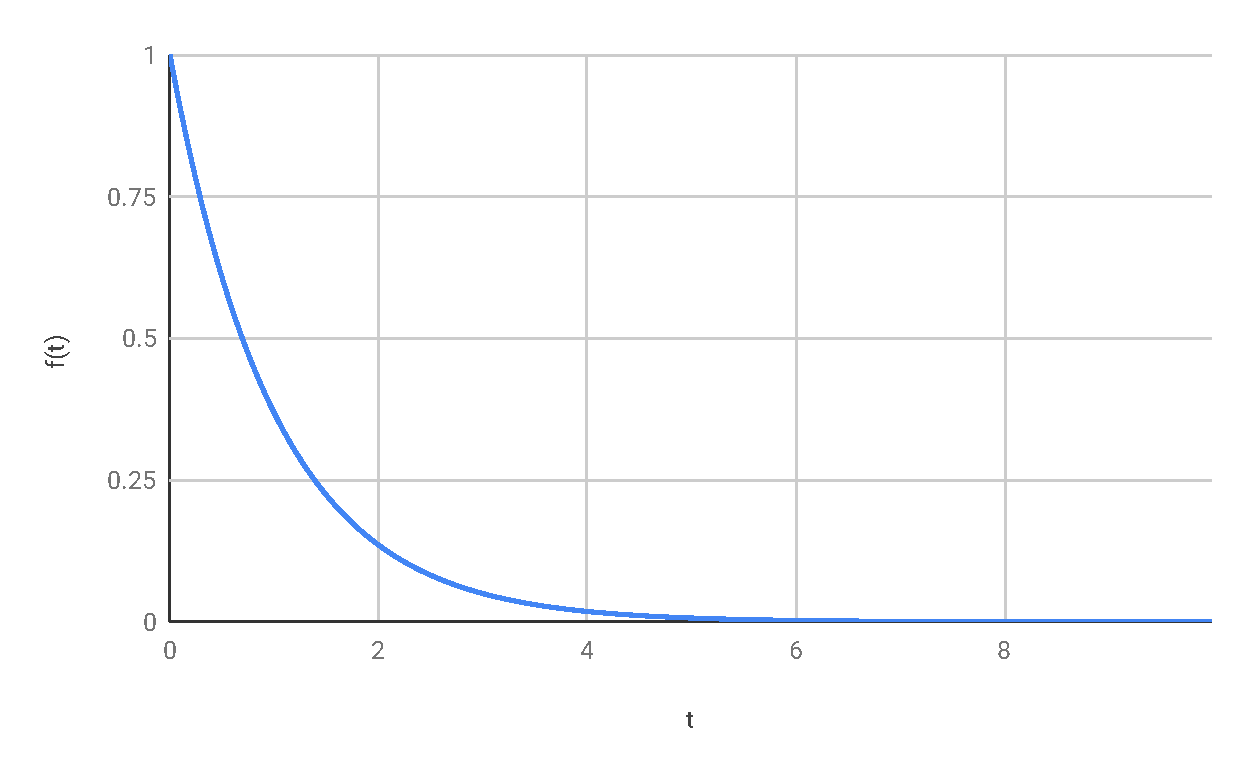
\includegraphics[scale=0.74]{image/05-RC-RL/f.pdf}
    \caption{Function $f(t)$}
    \label{figure.05.f}
\end{figure}
%%%%%%%%%%%%%%%%%%%%%%%%%%%%%%%%%%%%%%%%%%%%%%%%%%%%%%%%%%%%%%%%%%%%%%%%%%%%%%%%
\begin{figure}[ht]
    \centering
    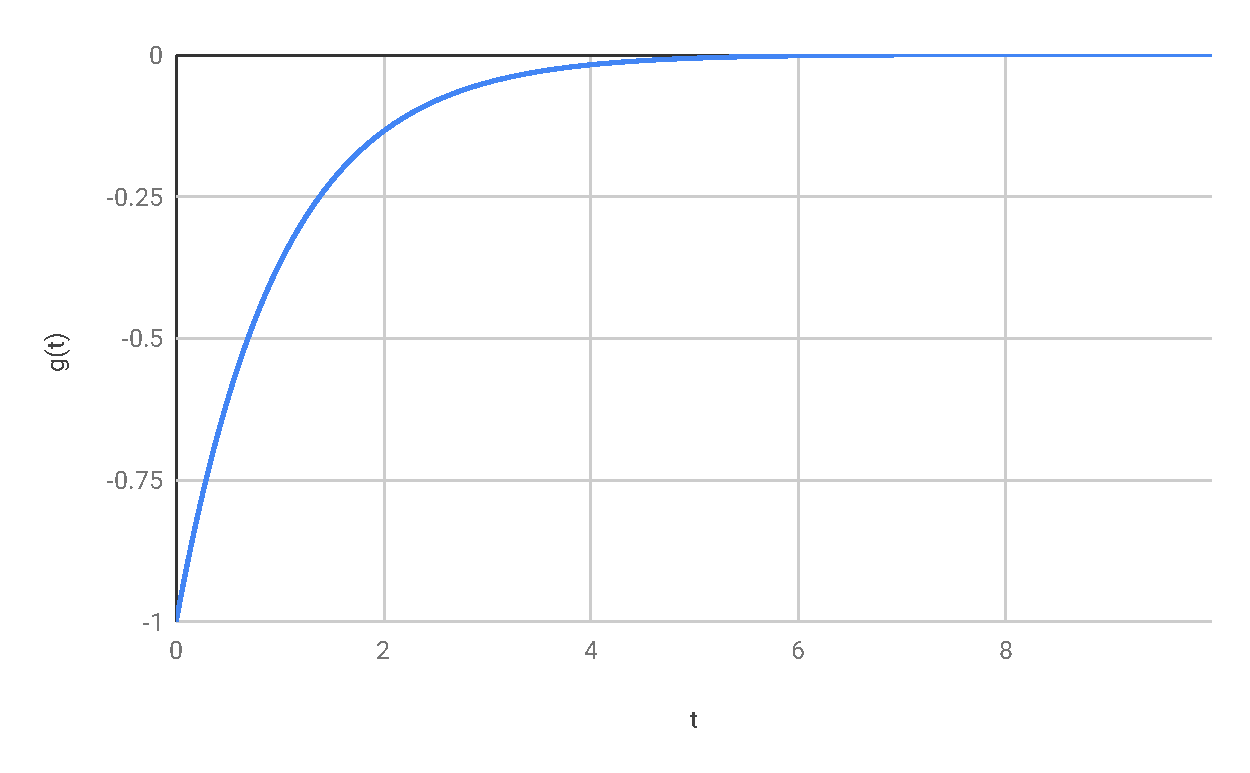
\includegraphics[scale=0.74]{image/05-RC-RL/g.pdf}
    \caption{Function $g(t)$}
    \label{figure.05.g}
\end{figure}
%%%%%%%%%%%%%%%%%%%%%%%%%%%%%%%%%%%%%%%%%%%%%%%%%%%%%%%%%%%%%%%%%%%%%%%%%%%%%%%%
\begin{figure}[ht]
    \centering
    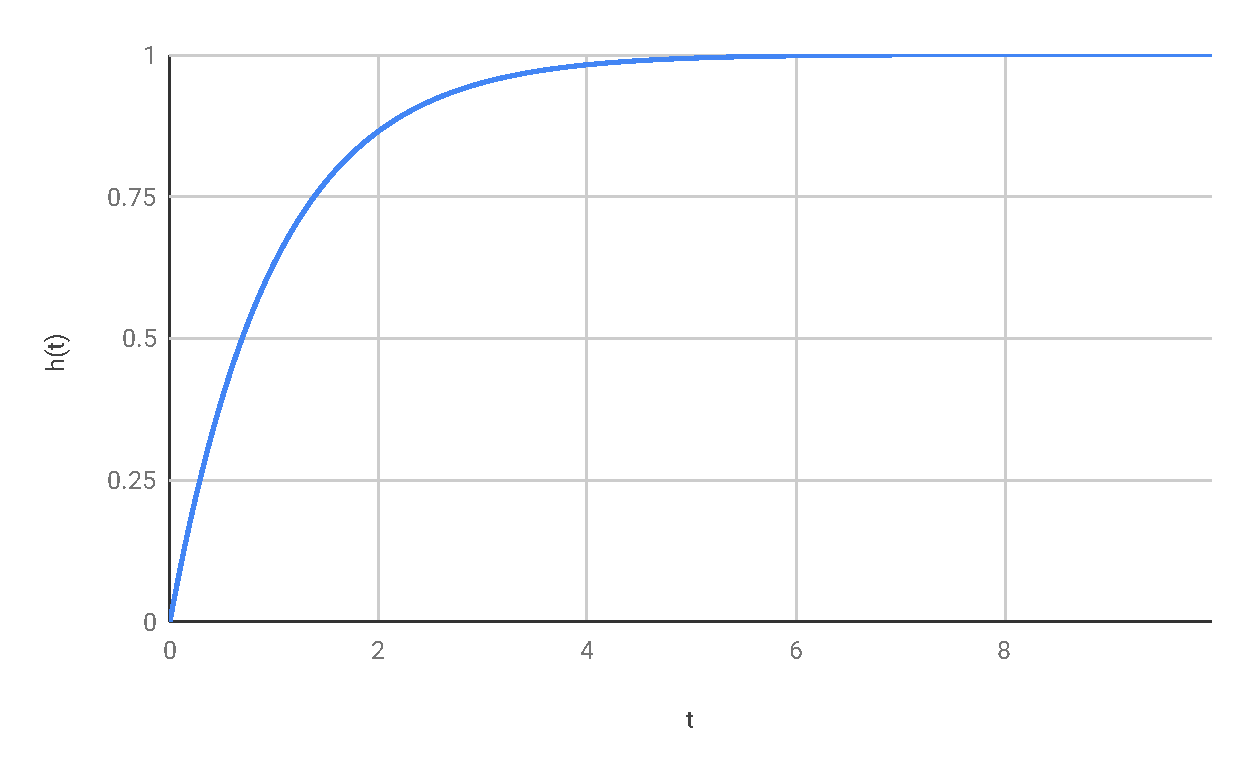
\includegraphics[scale=0.74]{image/05-RC-RL/h.pdf}
    \caption{Function $h(t)$}
    \label{figure.05.h}
\end{figure}
%%%%%%%%%%%%%%%%%%%%%%%%%%%%%%%%%%%%%%%%%%%%%%%%%%%%%%%%%%%%%%%%%%%%%%%%%%%%%%%%
\begin{figure}[ht]
    \centering
    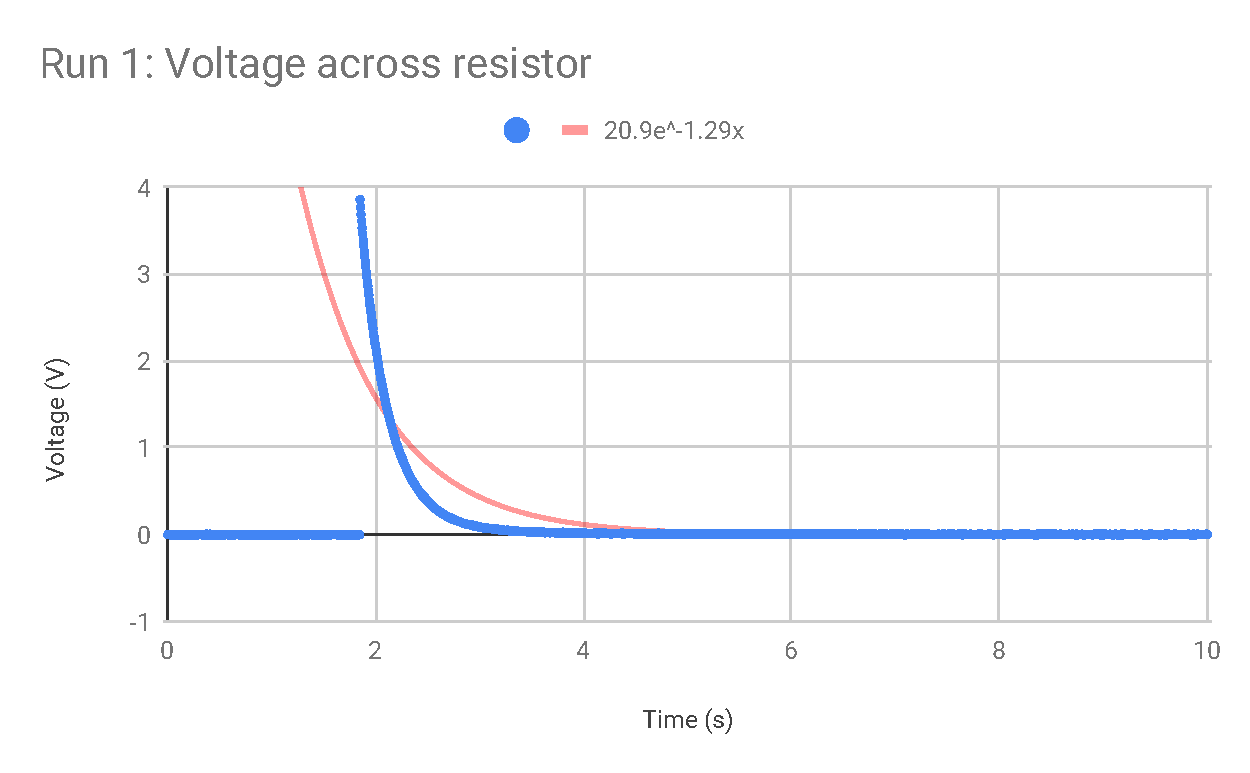
\includegraphics[scale=0.74]{image/05-RC-RL/run-1-vR-full.pdf}
    \caption{Run 1: $V_{R}(t)$}
    \label{figure.05.run.1.vR.full}
\end{figure}
%%%%%%%%%%%%%%%%%%%%%%%%%%%%%%%%%%%%%%%%%%%%%%%%%%%%%%%%%%%%%%%%%%%%%%%%%%%%%%%%
\begin{figure}[ht]
    \centering
    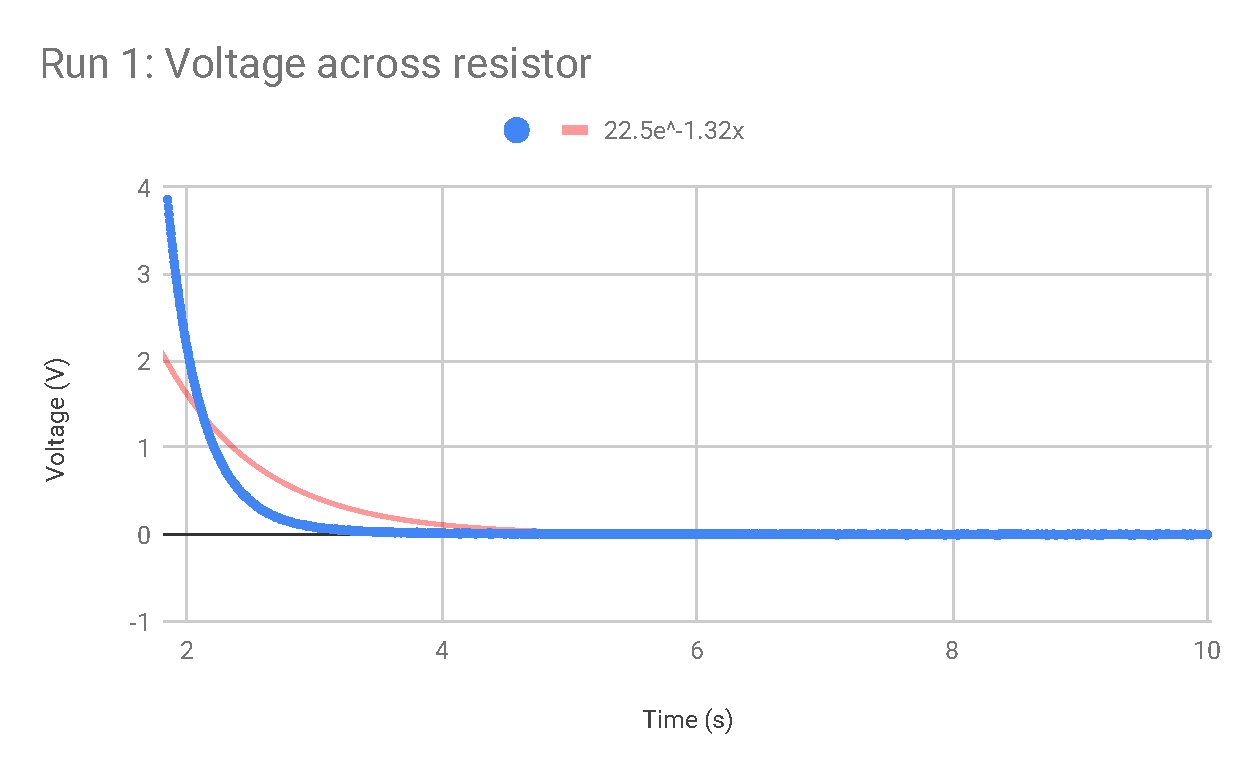
\includegraphics[scale=0.74]{image/05-RC-RL/run-1-vR-truncated.pdf}
    \caption{Run 1: $V_{R}(t)$}
    \label{figure.05.run.1.vR.truncated}
\end{figure}
%%%%%%%%%%%%%%%%%%%%%%%%%%%%%%%%%%%%%%%%%%%%%%%%%%%%%%%%%%%%%%%%%%%%%%%%%%%%%%%%
\begin{figure}[ht]
    \centering
    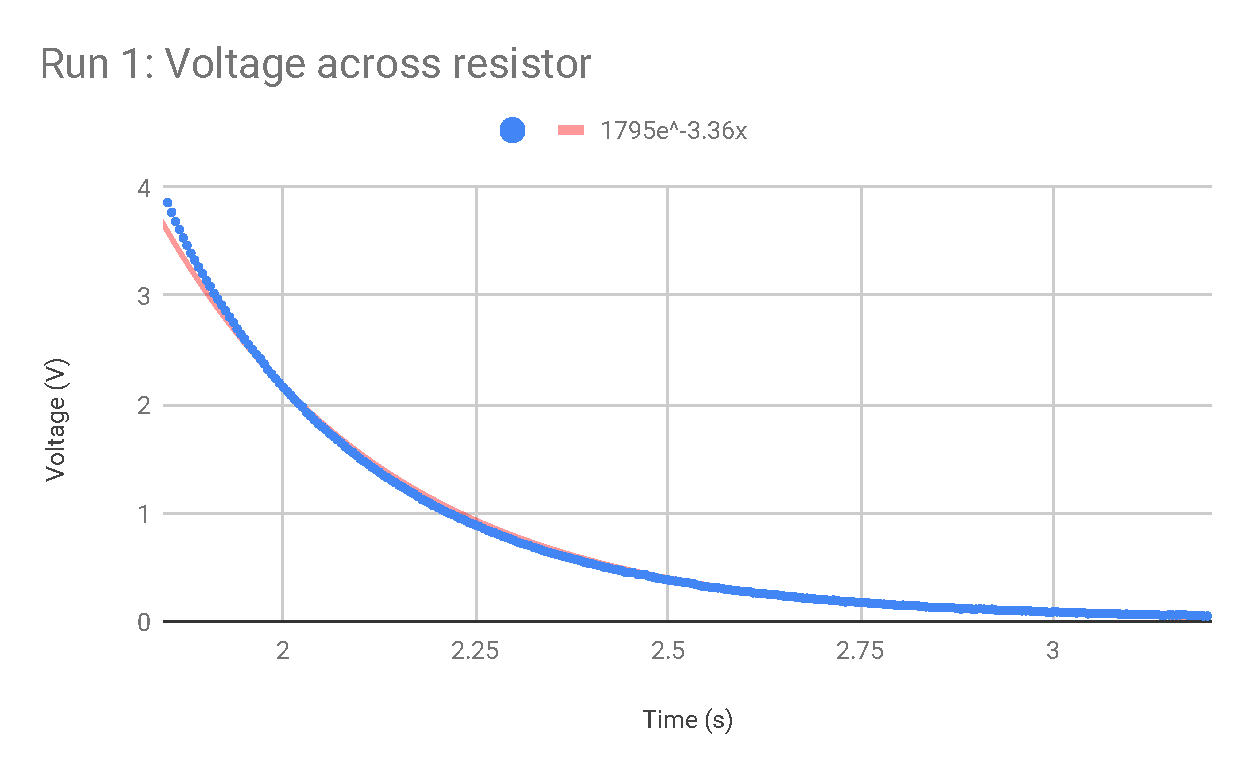
\includegraphics[scale=0.74]{image/05-RC-RL/run-1-vR-no-tail.pdf}
    \caption{Run 1: $V_{R}(t)$}
    \label{figure.05.run.1.vR.no.tail}
\end{figure}
%%%%%%%%%%%%%%%%%%%%%%%%%%%%%%%%%%%%%%%%%%%%%%%%%%%%%%%%%%%%%%%%%%%%%%%%%%%%%%%%
\begin{figure}[ht]
    \centering
    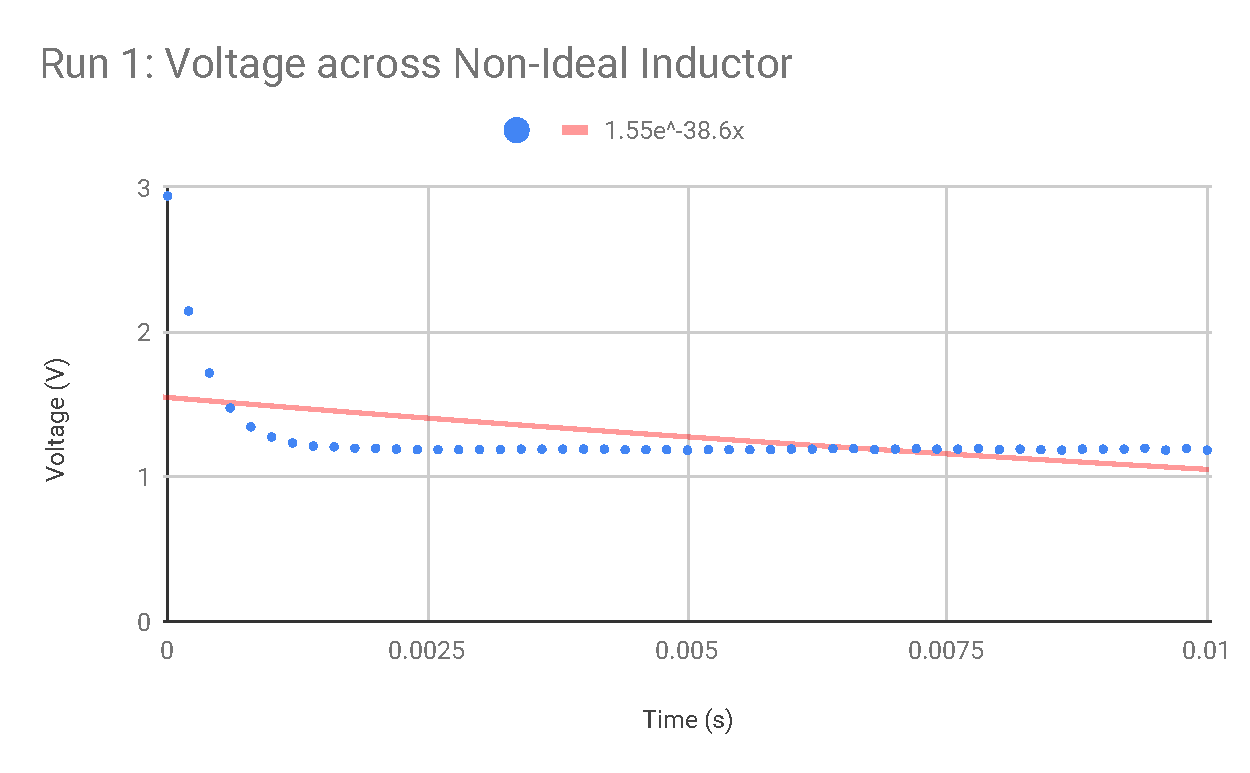
\includegraphics[scale=0.74]{image/05-RC-RL/vL-non-ideal-full.pdf}
    \caption{Run 1: $V_{r}(t) + V_{L}(t)$}
    \label{figure.05.vL.nonideal.full}
\end{figure}
%%%%%%%%%%%%%%%%%%%%%%%%%%%%%%%%%%%%%%%%%%%%%%%%%%%%%%%%%%%%%%%%%%%%%%%%%%%%%%%%
\begin{figure}[ht]
    \centering
    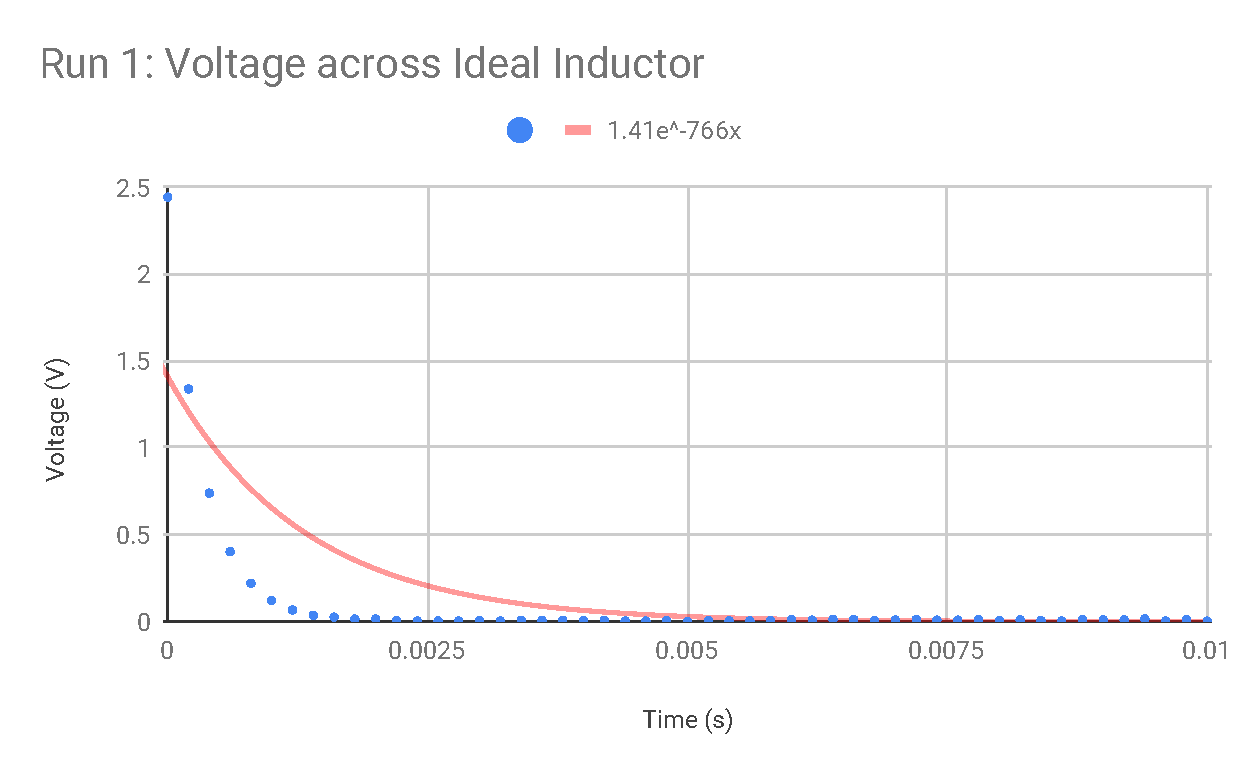
\includegraphics[scale=0.74]{image/05-RC-RL/vL-full.pdf}
    \caption{Run 1: $V_{L}(t)$}
    \label{figure.05.vL.full}
\end{figure}
%%%%%%%%%%%%%%%%%%%%%%%%%%%%%%%%%%%%%%%%%%%%%%%%%%%%%%%%%%%%%%%%%%%%%%%%%%%%%%%%
\begin{figure}[ht]
    \centering
    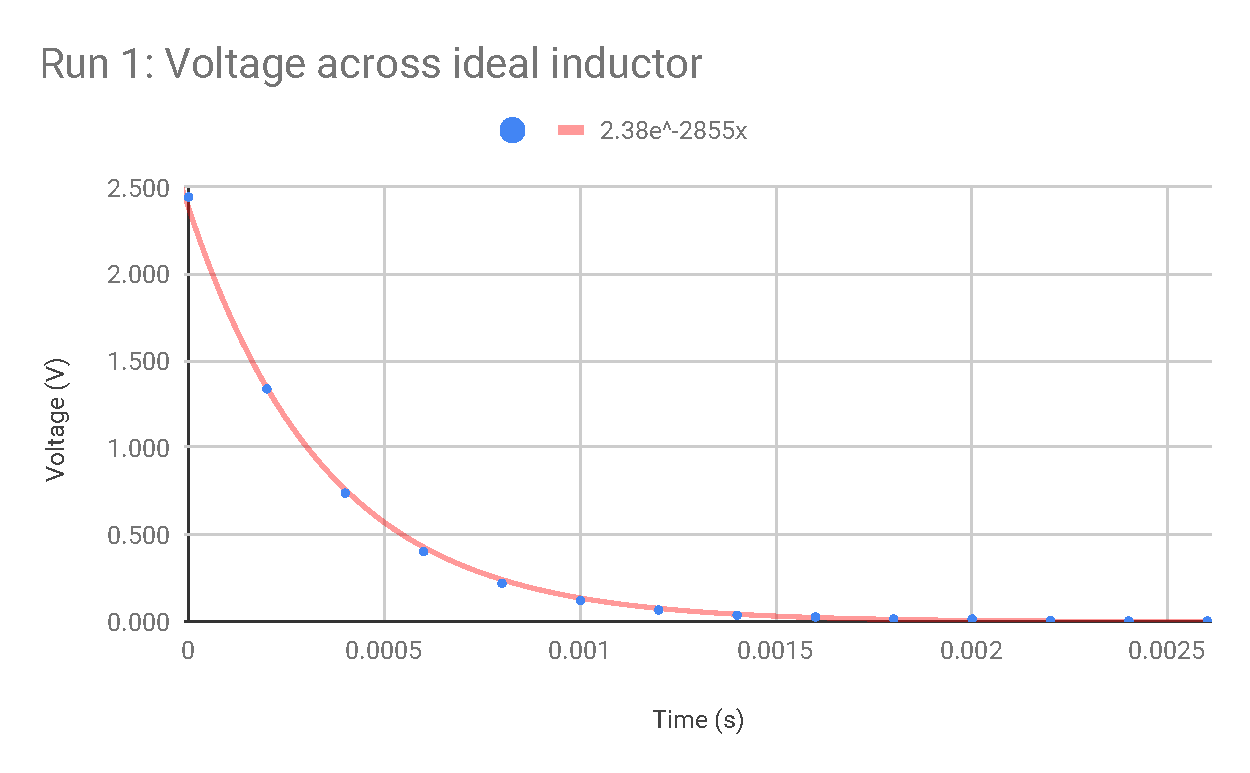
\includegraphics[scale=0.74]{image/05-RC-RL/run-1-vL.pdf}
    \caption{Run 1: $V_{L}(t)$}
    \label{figure.05.run.1.vL}
\end{figure}